\section{The single-time estimator as a functional of the track segment}\label{sec:formulation}

\subsection{What a strip sees}

Consider a straight track through a drift gap of length $L$, inclined by $\theta$ to the drift direction, read by strips of
pitch $p$ (\cref{fig:schematic}a). Charge released at depth $z$ drifts for $u = z/v$ and arrives at the readout plane at
transverse position $x(z) = x_0 + z\tan\theta$, spread laterally by a distribution $f(x - x(z); z)$ of width $\sigma(z)$. The
current on strip $i$ is the sum over depths of the fraction of each depth's charge that lands within the strip, each folded
with the electronics response $T$:
\begin{equation}
  W_i(t) = \int_0^{L/v} du\; q(u)\, F_i(u)\, T(t - t_0 - u), \qquad
  F_i(u) = \int_{x_i - p/2}^{x_i + p/2} f(x - x(vu); vu)\, dx .
  \label{eq:waveform}
\end{equation}
With no lateral spread, $F_i$ is a box: strip $i$ collects exactly the depths $z_i \le z < z_i + \Delta z$ with
$\Delta z = p/\tan\theta$, over a time $\Delta t = p/(v\tan\theta)$. With a spread, strip $i$ also receives charge from depths
outside its box, from a range of order $\sigma(z)/\tan\theta$ on either side.

A hit-based readout keeps one time per strip, $t_i = \mathcal{E}[W_i]$, where the estimator $\mathcal{E}$ is a threshold crossing,
a leading-edge fraction of the peak, the time of the peak, a fitted rising edge, a time over threshold, or a charge-weighted
mean. The $\mu$TPC then fits a line $t_i = t_0' + x_i/w$ through the hits and reads the slope $w = dx/dt$ as $v\tan\theta_{\rm rec}$.
For an interior strip, with charge from both neighbouring depths on both sides, every estimator returns the time of some
representative depth within the strip's box, shifted by an amount that is the same for every interior strip when the spread is
the same at every depth: the interior ladder keeps its slope and only its offset moves. This is the first result of the
formulation and the reason a charge-weighted time, a peak time and a leading edge all give nearly the same angle: the
estimator cannot change the slope of a translation-invariant ladder.

Three things break the invariance.

\paragraph{The partial end strips.} The strip through which the track enters the gap collects charge only from $z = 0$ to the
strip's far edge, a fraction $\phi$ of a full box; the strip through which it leaves collects the complementary fraction. Their
charge is less, and their time is that of a shorter and one-sided column, while the fit assigns them the strip centre. For the
entry strip the estimated time is later than the interior line extrapolated to the strip centre by about $(1-c)(1-\phi)\Delta t$,
for the exit strip earlier by about $c(1-\phi')\Delta t$, where $c$ is the fraction of the column at which the estimator reads
(0.3 for a 30\,\% leading edge, 0.5 for a centroid). Averaged over entry phases the two ends are displaced in opposite
directions by a fixed fraction of $\Delta t$. This is the ``edge-strip position'' effect named by Bortfeldt~\cite{Bortfeldt2015}
and the ``purely geometrical'' bias of Ntekas's gas-only simulation~\cite{Ntekas2016}; it exists with no lateral spread at all.

\paragraph{The ghost strips.} A strip whose centre lies outside the track's projection receives charge only through the
lateral spread. At the mesh end its charge comes from the shallowest depths and its time is close to $t_0$, later than the line
extrapolated to its position; at the cathode end its charge comes from the deepest depths and its time is earlier than the
line. Both displacements rotate the fitted line toward smaller $dt/dx$, i.e.\ toward a steeper track. The published ``ghost
hit'' of the capacitive-coupling literature~\cite{Farinelli2019,Ntekas2016} is this strip; a Gaussian footprint, drift
diffusion and resistive spreading produce it equally.

\paragraph{A spread that grows with depth.} If $\sigma$ grows with $z$ the shift of an interior strip's estimated time is no
longer the same at every depth. For a leading-edge estimator the earliest substantial charge on a strip comes from shallower
depths through the spread, by about $\sigma(z)/(v\tan\theta)$ in time, so the deeper strips are pulled earlier by more than the
shallower ones and the interior ladder itself is compressed. For a charge-weighted time the first-order effect cancels: the
mean of a symmetric spread is the strip centre, and the growth of the width enters only through the gradient of $\sigma^2$,
which gives a depth-independent offset $D^2/\tan^2\theta$ and no slope change~\cite{paperII}. \Cref{sec:toy} verifies both
statements numerically.

\subsection{The scaling}\label{sec:scaling}

Displacing the two end points of a least-squares line through $N$ equally spaced points by $\pm\delta$ in time changes its
slope by $12\delta/(N(N+1)\Delta t)$ (\cref{app:endterm}). Since both the partial strips and the ghosts move the ends by
amounts of order $\Delta t$ (geometry) or $\sigma/(v\tan\theta)$ (spread), the ratio takes the form
\begin{equation}
  \frac{\tan\theta_{\rm rec}}{\tan\theta} - 1 \;\simeq\; \frac{C}{N^2} + b, \qquad N = \frac{L\tan\theta}{p},
  \label{eq:scaling}
\end{equation}
where $C$ collects the end displacements in units of $\Delta t$ (geometry gives $C$ of order 1 to 2; each lateral spread adds a
term that grows with $\sigma/p$) and $b$ is the interior compression from the depth-growing spread, of order
$c\,D_T/(2\sqrt{z}\tan\theta)$ for a leading edge and zero for a centroid. In terms of the slope, $\Delta\tan\theta = a/\tan\theta +
b\tan\theta$ with $a = C(p/L)^2$. Three consequences follow and are tested below:

\begin{enumerate}
\item The bias is large at small angles and falls as $1/\tan^2\theta$: the shape every strip-$\mu$TPC study reports, and the
  reason it was treated as a calibration. It is a property of the number of strips in the column, not of the angle as such.
\item At fixed angle it grows with the pitch, through $N$ and through $C$, so coarser readout makes it worse, not better.
\item It depends on the estimator only through $C$ and $b$; a change of estimator or threshold cannot remove it, and a
  charge-weighted time removes only the interior part $b$, which is small whenever the column is a few strips long.
\end{enumerate}

The transparent toy of \cref{app:toy} gives $C$ a closed form for an amplitude-weighted leading-edge ladder: over
thirteen configurations spanning footprints of 0.07 to \SI{0.45}{mm}, diffusion on or off and pitches of 0.39 to \SI{1.56}{mm},
\begin{equation}
  C \;\simeq\; 1.1 + 11\,\Big(\frac{\sigma_{\rm rms}}{p}\Big)^2, \qquad \sigma_{\rm rms}^2 = \sigma_0^2 + \tfrac{1}{2} D_T^2 L,
  \label{eq:Claw}
\end{equation}
with a residual of 0.06 in $C$ ($\sigma_{\rm rms}$ is the lateral spread averaged over the column; the spread at full drift
fits six times worse). The constant is the strip geometry; the quadratic term is the ghost strips, whose charge and whose lever
arm both grow with the spread. Other estimators move $C$ by $\pm 20\,\%$ at fixed spread (\cref{tab:estimators}).

Two dimensionless numbers therefore decide whether a readout will see the effect: $N$, the strips in the column, and
$\sigma_\perp/p$, the total lateral spread in units of the pitch, with $\sigma_\perp^2 = \sigma_0^2 + D_T^2 L$ at full drift.
The equivalent statement used in the pad-TPC literature is the lever arm $\Lambda = \sigma_T(L)/(L\tan\theta)$, the mixing width
over the projected column; $\Lambda = (\sigma_T/p)/N$, so the two formulations carry the same information and \cref{eq:scaling}
is the more useful one because it separates the two factors.

\begin{figure}[t]
  \centering
  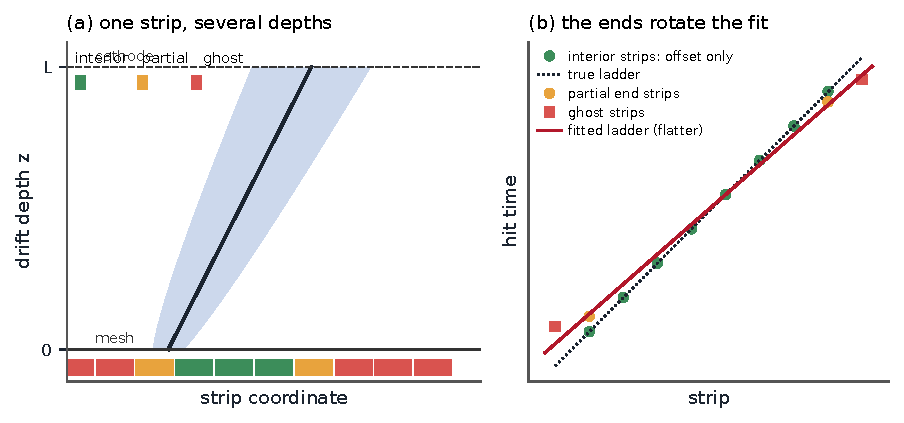
\includegraphics[width=\linewidth]{schematic}
  \caption{(a) A strip reads the charge of several drift depths: the interior strips (green) collect a full box of depths, the
  two partial strips at the ends of the column (orange) a fraction of one, and the ghost strips (red) only what the lateral
  spread (shaded) brings them. (b) In the ladder of one time per strip, the interior strips keep the true slope and move
  together; the partial strips and the ghosts are displaced in opposite directions at the two ends and rotate the fitted
  line toward a steeper track.}
  \label{fig:schematic}
\end{figure}
